\documentclass[12pt]{article}

\setlength\parindent{30pt}
\usepackage[usenames, dvipsnames]{color}
\usepackage{fullpage}
\usepackage{setspace}
\usepackage{amssymb}
\usepackage{amsmath}
\usepackage{caption}
\usepackage{subcaption}
\usepackage{graphicx}
\usepackage[section]{placeins}
\usepackage[utf8]{inputenc}
\usepackage[T1]{fontenc}

\doublespacing


\newcommand{\TODO}[1]{\textcolor{red}{#1}}
\newcommand{\F}[1]{\textcolor{magenta}{#1}}

\newcommand{\contradiction}{{\hbox{%
      \setbox0=\hbox{$\mkern-3mu\times\mkern-3mu$}%
      \setbox1=\hbox to0pt{\hss$\times$\hss}%
      \copy0\raisebox{0.5\wd0}{\copy1}\raisebox{-0.5\wd0}{\box1}\box0
    }}}


\newcommand\Nbb{\mathbb{N}}
\newcommand\Pbb{\mathbb{P}}
\newcommand\Zbb{\mathbb{Z}}
\newcommand\Rbb{\mathbb{R}}
\newcommand\Mcl{\mathcal{M}}

\begin{document}
\title{CMSC 234}
\author{Patrick Collins, Zachary Jenkins \& Mark Landgrebe}
\date{\today}
\maketitle
\pagebreak

\section{Contact Info}
Team Name: PlayListr

\begin{center}
\begin{tabular}{l|l}
 Member           &  Email                    \\ \hline
 Patrick Collins  &  pscollins@uchicago.edu   \\
 Zachary Jenkins  &  zjenkins@uchicago.edu    \\
 Mark Landgrebe   &  mlandgrebe@uchicago.edu  \\
\end{tabular}
\end{center}

\pagebreak

\section{Motivation}

There are two main objectives that we wish to accomplish with our
mobile and wearable Android application Playlistr. Our first objective
is to democratize control of the music-playing experience at casual
hangouts, parties, and bars and cafes. Our second main objective is to
collect sensor data from the surroundings, particularly of users’
physical movements and heart rate, in order to learn about users’
music listening preferences and to recommend music based on these
perceived preferences. By focusing on these two objectives, we will
explore many of the ideas that we have explored in class, such as
“Ubiquitous Computing” and “Everyware”, and we will develop software
for the latest Android devices, including Android smart watches and
new Android mobile smartphones.

The “Background/Prior Work” section of this write-up provides a
description as to why we want to democratize music selection in a
group setting, and this section describes the research and ideas that
our application will incorporate and how our application could
potentially show proof for these various concepts. Broadly speaking,
Playlistr will allow users to queue up songs from their own mobile
devices to a central device, which would presumably be connected to
speakers and would be playing music on a central playlist, at the
event. In addition, we will provide additional features, such as
voting and starring songs, in an effort to give users even more
influence over the music. Initially, we thought that these key
features could make for a great music application and potentially
change the music-playing experience in various group
settings. However, having been exposed to many papers concerning
mobile computing in this course, we now believe that we can create a
much better application. Playlistr is based, in part, on the ideas of
Weiser and Greenfield and on one ubiquitous computing vision that we
discussed in class, which envisions an environment that constantly
adjusts based on peoples’ preferences, which are pulled from their
smartphones, wearables, etc. When one first conceives an idea for an
application that he or she thinks could solve a problem or fill some
need, one might have the tendency to overestimate the extent to which
new users would be willing to explicitly interact with the application
in order to fill a need. In our case, we believe that we have
identified a problem with music-playing in group settings, but we are
no longer confident that a large number of users would be willing to
frequently queue songs and have to press buttons to vote for songs on
the central playlist. These features will still be very much a part of
our application, as they will allow users who are willing to interact
directly with our application to precisely share their music listening
preferences with the group. However, we believe that there needs to be
a way for more-passive users to be able to share their preferences
with the group with very little effort on their part.

Let us consider the popular music application Pandora with its voting
system, which requires users to physically press/click vote buttons in
order to help the service better select music for the
listener. Pandora's music selection algorithms are extremely
sophisticated and, in our opinion, quite good at selecting music for
users when they listen by themselves. However, we find it puzzling
that the only way for users to relay their preferences to Pandora is
for them to press voting buttons. We live in a world where "The
Internet of Everything" is the latest phenomenon. There are many smart
devices that determine users’ preferences passively, such as
thermostats, notably Nest thermostats, which regulate temperature in
homes by collecting data from the surrounding environment and
analyzing patterns in this data to conform to users’ preferences and
save them money on energy when they are not around. Our application
develops Greenfield’s belief, “Surfaces, gestures, behaviors as we've
seen, all have become fair game for technological intervention” and
focuses on using peoples’ gestures and behaviors, in response to
music, to gage their music-listening preferences. By using
accelerometers to measure peoples’ varying levels of activity during
songs and by collecting heart rate data, we will complement our more
traditional, explicit, voting and queuing systems. Users will not have
to press buttons to give their feedback on the music, but rather will
need to just open up Playlistr at an event and allow it to collect
data on how they respond to the music.

We believe that it is crucial to support Android wearables in addition
to Android smartphones. We will need to rigorously test our
application on both types of devices, in order to determine how
accurately wearables and smartphones can collect sensor data. With
wearables, we believe that we can collect accurate information on
groups of users at particular events and potentially give better
recommendations for songs to play in particular groups than those of
services like Pandora or Rdio. In our opinion, some songs are better
for parties, dancing, drinking, etc., and we do not believe that
services like Pandora and Rdio, which rely on their push-button voting
system, understand this as well as they could if they were to analyze
the movements and vitals of their users. If time permits, we would
like to use the sensor data that we collect to facilitate user
interactions at events. This could involve something as simple as
sending push notifications to two users whose activity levels are low
and suggesting that they dance together. We are interested in
exploring more possibilities for facilitating user interaction after
we have the main functionality for our application working. Not only
will we use sensors to collect information on a user’s reaction to
music, but we will also rely on a user’s location to make it easy for
users to learn about and join “SongRooms”, which hold a group’s
collaborative playlist. In working on this application, we will learn
more about the capabilities of current mobile technologies to collect
sensor data, and we will create a music application that changes the
way music is selected in group settings, making it easy for both
active and passive listeners to have a say in what is played.

\pagebreak
\section{Background}

At events where music is played, guests have limited control over song
selection. This creates several problems. When a guest has a song
request, he or she can plug their phone into the speaker system and
annoy the entire party, pester the host or DJ into playing a song, or
remain dissatisfied. None of these is an optimal event experience for
anyone involved. Moreover, event-goers have no way of getting the
playlist of the songs played at the party.

It is in everyone’s best interest to ensure that these problems are
dealt with. If people are having suboptimal experiences at parties,
bars, and other venues, they will be less inclined to spend more time
and money there.

Playlistr gives the host of an event the ability to create a SongRoom,
which will hold a central playlist that people can join as
guests. When a host creates a SongRoom, he or she chooses one of his
or her Spotify playlists, or an empty playlist, and this playlist
becomes central to the party, allowing guests to add songs to it and
vote for songs on it. The host will be given certain administrative
privileges within the SongRoom, such as the ability to remove users
from the SongRoom, the ability to remove songs from the playlist, and
the ability to skip songs and play any songs, even if they are not on
the playlist, whenever he or she chooses. The music will play on the
host’s phone, which will presumably be connected to speakers.

Users will be able to queue songs from their Spotify playlists and
song libraries. In addition, users will be able to see the song that
is currently playing and those on the queue that will be played
later. Finally, users will have many other capabilities, including the
ability to vote on songs in the queue, so that they can give priority
to songs that they want to hear most at these events. All of the
features that have been described so far can be done on
smartphones. There are even more features that will be available to
users who own an Android smart watch. These users will be able to use
their smartwatches as extensions of a smartphone application The
smartwatch application that we will build will be a pared-down version
of the smartphone app, with the exception of added functionality for
collecting sensor information about its wearers, particularly heart
rate data and motion data. To be clear, the Playlistr application that
runs on Android smartwatches will support voting, will allow users to
vote for songs on the main playlist, and will collect their movements
and heart rate in order for the application to passively learn about
their listening preferences. The application will process the sensor
information it receives from users and make song predictions based on
music that presumably caused an increase in physical activity, as
measured with accelerometers and heart rate sensors. If time permits,
we would like to use these data to facilitate user interaction in
clever ways. In the motivation section, we said how this could be as
simple as sending push notifications to two users whose activity
levels are low and suggesting that they dance together. This
application will give users with smartwatches the ability to influence
the music that plays without having to necessarily vote for songs by
pressing buttons.

Most of Playlistr’s competitors are really indirect
competitors. Preexisting music services that people currently use to
listen to music fall under this category. These services include
iTunes, Pandora, Youtube, Soundcloud, and even Spotify. None of these
services provides the ability to collaboratively manage a playlist
during a party, but many people currently use some combination of
these services to handle a party’s music. These services have very
large user bases – virtually all music listeners use them today. In
fact, the most significant challenge in getting party hosts to use our
app will be to get them to change their behavior – using Playlistr
will let hosts ensure that their guests have a better time by having a
little more control over the music, without any extra mental overhead
on the host’s part.

Each of these services also has special licensing agreements with
different record labels–a significant barrier to entry for new
services. By using Spotify’s API, we can ensure that users have access
to all 30 million songs available on the platform. This is well within
their terms of service, and since we incentivize people to join
Spotify (by requiring them to login through Spotify O-Auth if they
want to play songs or save songs), this is beneficial to their
business, too.

Crowdcast, Sonos, and Spotify Connect are more-direct
competitors. Crowdcast is an iOS app that attempts to accomplish a
very similar task – collaborative playlist management. However, they
approach it very differently from what we plan. They attempt to
license their own music, which makes users responsible for paying for
the rights to songs. The users must already own or purchase the songs
on iTunes in order to queue them up in the collective playlist. This
works for people with extensive iTunes collections, but many
individuals now use streaming services in order to get their music. By
using Spotify’s API, we provide access to all of their songs for
free. Moreover, Crowdcast is only usable on iOS devices, and requires
use of Bluetooth-enabled multi-peer connectivity. By the user specs,
this is limited to eight devices, and so is not really applicable to
larger groups.

Sonos is a Bluetooth-enabled speaker system that connects directly to
phones. A phone connected via Bluetooth to the speakers will stream
all audio directly to them. Only one person can connect to a Sonos
speaker at any given time, but multiple people can have access to
them. In this way, partygoers can switch control of the speakers
between themselves. There is no central playlist for the Sonos
speakers, though, so people not currently connected to the speakers
have no way of influencing what music is played. Also, there could be
other issues with having guests take control over music- playing, such
as not being able to give one user, such as the host of the event,
certain administrative abilities, or running into issues where a user
takes over control of playing music and does not have good cell
reception or does not have access to a good Wi-Fi network, which could
cause interruptions in the music and a reduction in music
quality. Moreover, the speakers are expensive and venues that have
already invested in a sound system will likely not want to switch over
to Sonos. Spotify Connect, on the other hand, supports a very similar
use case, but does not require specific speakers.  Rather, it requires
only a music-playing device that can run the Spotify/Spotify Connect
app. Spotify Connect can be a more affordable alternative to Sonos,
but has the same issues, such as limiting control of the music to the
individual who is currently paired with the device running the
Spotify/Spotify Connect app and the potential problems with switching
between users with different cellular providers and with different
access to Wi-Fi networks.

Overall, this has been a broad overview of the various features of
Playlistr and the competition the application will face. The
application will be described in more detail in the following sections
with the aid of various diagrams that should give the reader a better
idea of the appearance of the application on the frontend and what the
backend infrastructure will include.



\pagebreak

\section{Project Specification}
The fundamental purpose of PlayListr is to improve the experience of
guests at events playing music. However, there are a variety of
avenues by which we can achieve this goal, and we hope to explore as
many of them as we can under the time constraints.

\subsection{Capabilities}
We can divide our planned features in to a hierarchy, such that each
higher level depends upon a correct implementation of the previous
one:

\begin{enumerate}
\item Core functionality.

The core functionality of the app is to allow a host to create a ``room,''
and to allow guests who join the room to have control over the music
that is played.

However, a variety of structure must be in place in order to
accomplish this goal. The core functionality is the most ambitious
part of this project --- a successful implementation requires:
\begin{itemize}
\item Correct interoperation with Spotify in order to authenticate
  users and stream music.
\item Construction of a database to hold identifying information about
  users, with sufficient information to reconstruct the user's Spotify
  account details, as well as the details of all existing rooms and
  the songs enqueued within them.
\item Development of a server that exposes a REST API, giving access
  to the database and allowing simple CRUD operations.
\item Ensuring consistency across many mobile users connected to the
  same room, taking in to account the possibility of high network
  latency over cellular data networks.
\end{itemize}

With this in mind, we have focused our current development efforts on
building the core functionality before tackling the features that
follow --- in the ``software architecture'' section below, we outline
an implementation of the core functionality.

\item Location awareness.

Users should be prompted to join a room whenever they come within a
pre-set distance of an existing room via push notification.

\item Smartwatch integration.

  Users should be able to vote on songs and see the currently playing
  song from the display of their Android smartwatches. This will
  likely take place via Bluetooth communication with their
  smartphones. This step is crucial for the following step since
  smartwatch sensor data will allow for a much more accurate picture
  of user activity within a room.

\item Adaptive song selection on the basis of sensor data.

The app should detect when the activity level within a room rises or
falls and play faster- or slower-paced music, accordingly. For
simplicity, we will simply select songs currently in the queue and pad
tempo-matched songs with artificial votes in order to float them to
the top of the queue --- this avoids problems of trying to match the
genre of the music currently being played.

We can take a variety of angles in processing sensor data, but the
simplest is likely to be taking the average norm of the acceleration
vector of each user per unit time. For example, given that we have
accelerometer data for the user's acceleration $\vec{a}$ such that:
\[
\vec{a} = (x, y, z)
\]
And, letting $\vec{a}_u$ represent the acceleration vector for the user
$u$ belonging to the group of users $U$ in a room during the previous
tick, we define the activity level $l$ of that tick to be:
\begin{align*}
  l &= \sum_{u \in U} \frac{||\vec{a}||}{|U|}\\
  &= \sum_{u \in U} \frac{\sqrt{x^2 + y^2 + z^2}}{|U|}
\end{align*}
Yielding a natural and intuitive notion of ``activity level'' that can
be quickly computed.


\item Social features.

Users have a ``friend list,'' consisting of other users, that allows
them to initiate communication (perhaps via a builtin messaging
service, or a tie in to an external messaging service, such as
Facebook Messenger).

\item Gesture recognition.

Users can add each other to their friend lists by shaking hands. Time
permitting, we can explore other gestures, such as a high five to
indicate that both users upvote the current song.

\item User pairing on the basis of activity level.

Given that the server will have access to the activity levels of all
users in a room, users can opt-in to a ``friendly mode'' in which they
will be periodically asked if they would like to become friends with
another user in the room based on similar activity levels (and perhaps
similar music preferences). If both users accept, then a conversation
is initiated between the two.

\end{enumerate}

\subsection{Software Architecture \& Design}
\begin{figure}[h]
  \centering
  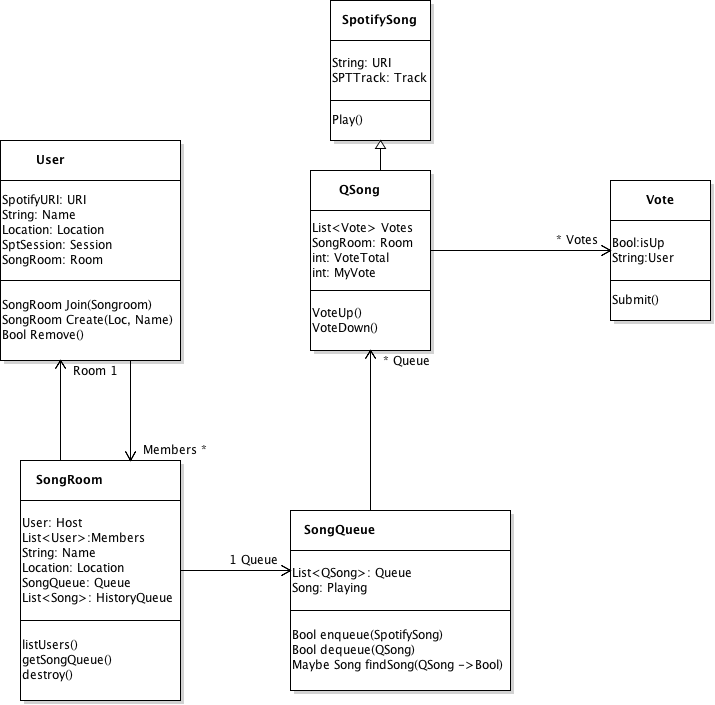
\includegraphics[width=4in]{ClassDiagram}
  \caption {UML Diagram of Client-Side Code}
\end{figure}


\begin{figure}[htb!]
  \centering
  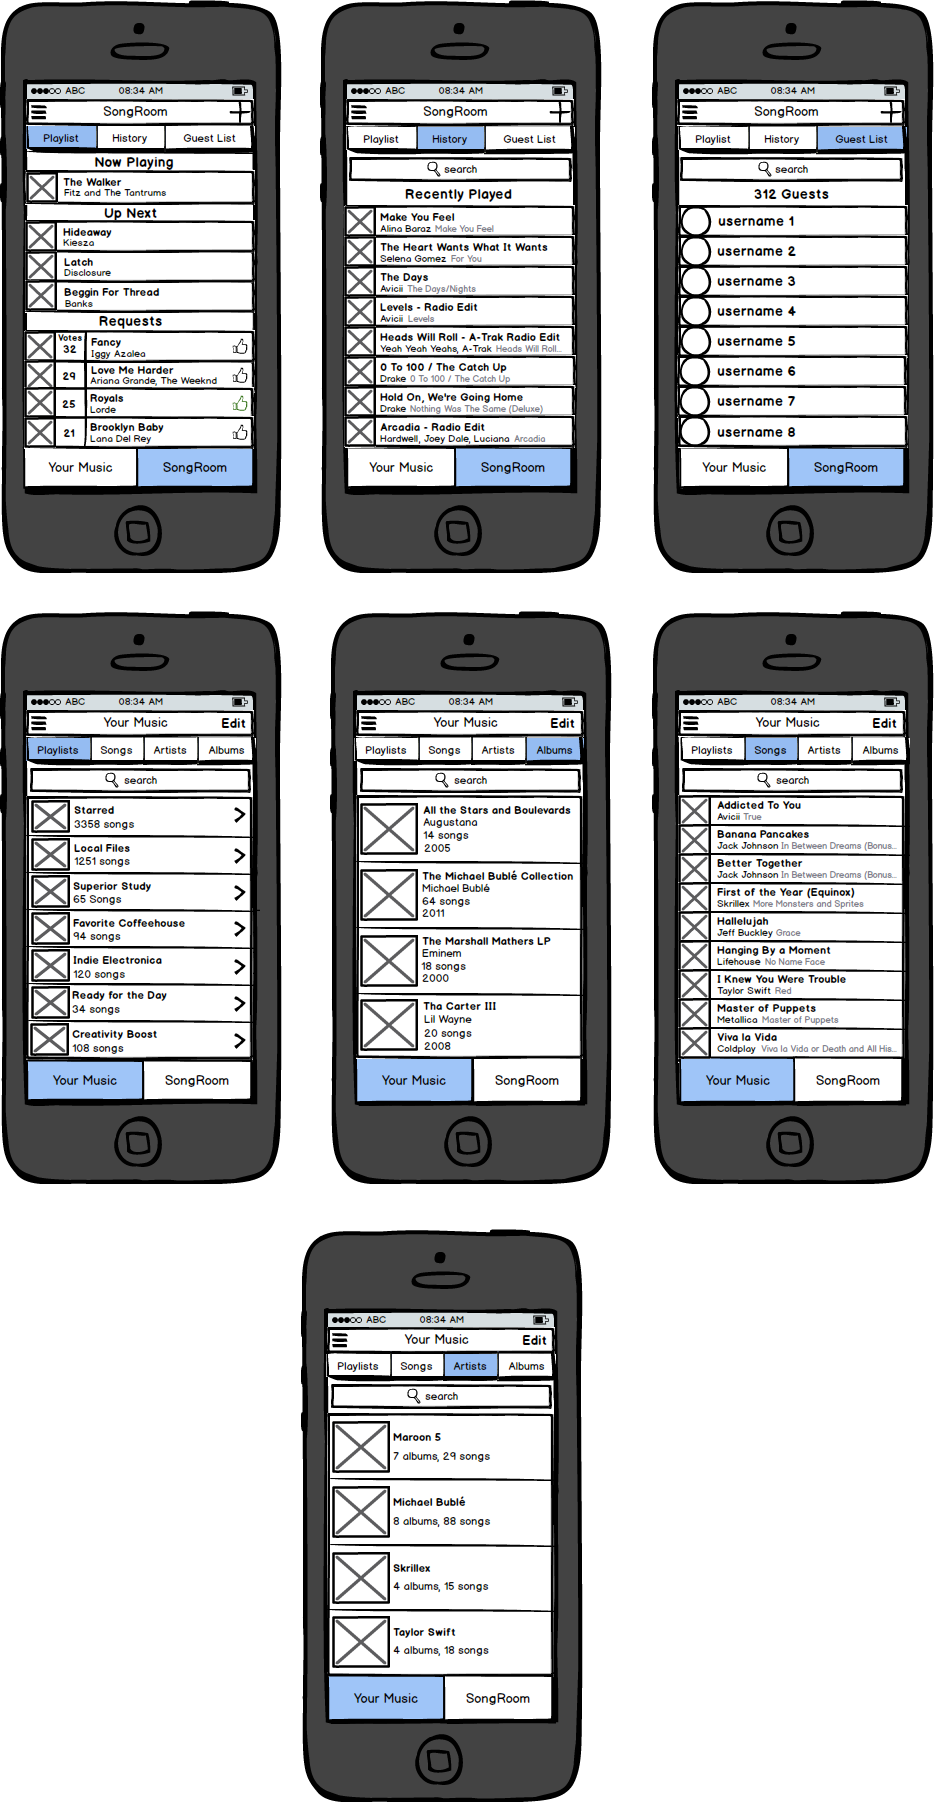
\includegraphics[width=4in]{mockup.png}
  \caption {UI Mockup}
\end{figure}

\begin{figure}[htb!]
  \centering
  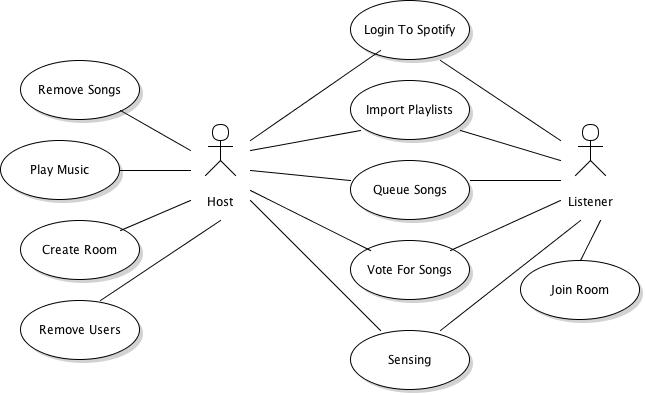
\includegraphics[width=4in]{usecase-diagram}
  \caption {Use Case Diagram}
\end{figure}


\pagebreak

\section{Planned Demonstration}

At the moment our demonstration is tough to solidify because at the
moment we do not know how sensing will play into our final project.
This will only become solidified when we learn more about how we can
use sensing to infer a users musical preference. However we think the
other usecases in the UML Usecase diagram below can be displayed
easily through a 3 phone interaction with 1 host and 2 Listeners. The
sensing element will likely require some sort of data visualization to
show how sensing influenced the most recent song. This is something
that we will further decide when we know what the nature of our
sensing usage will be.

\pagebreak

\section{Implementation Schedule \& Supporting Tools}

\subsection{Toolchain}

Tools: At the moment we plan on using several frameworks and APIs to
make our project happen. The Spotify Framework is how we will be
getting access to music streaming. The Flask Framework is a Python web
framework, which we will use for our server. We will also use the
Flask framework to allow our server to interface with a MongoDB
database using the Flask MongoEngine. The server and database will be
hosted on Heroku. For using music preference to choose music we plan
on using the Echo Nest API.

\subsection{Schedule}
Our first week we plan on working to get the basic functionality
working. Our plan for dividing the work is roughly:

\begin{itemize}
\item Mark --- Spotify (login to Spotify, play songs, import playlists)
\item Patrick --- Client Classes (create room, join room, enqueue/dequeue, upvote/downvote)
\item Zach --- Server (basic database structure,  location based room lookup)
\end{itemize}


Once we have the basic functionality our focus will shift in 2 ways
for the next week: get a basic UI working, figure out in what ways we
can use sensing through experimenting with the technology.


At the end of the second week (Sunday) we should have a rudimentary
version of the app working and an idea of what we want the final app
to look like. From here the rest should be implementation that we are
able to complete using our one-week iteration structure (Sunday to
Sunday.)

\end{document}
